\chapter{Resultados e Discussões}
\label{cap:resultados}

Neste capítulo são apresentados os resultados empíricos obtidos na validação da aplicação \textit{PON Planner}, acompanhados da análise crítica dos dados, da comparação com soluções correlatas descritas na literatura e da verificação sistemática do cumprimento dos objetivos estabelecidos para o trabalho.

\section{Apresentação dos Resultados}
\label{sec:apresentacao_resultados}

A coleta de dados empíricos foi estruturada para avaliar o desempenho computacional do \textit{backend}, a precisão física dos algoritmos de atenuação e o ganho de produtividade no planejamento de redes de acesso \gls{gpon}. Os cenários experimentais contemplam dois estudos de caso representativos de diferentes realidades de implantação física: uma rede em área urbana com topologia simétrica/balanceada e uma rede em área rural com topologia linear desbalanceada de longo alcance.

Essa distinção é fundamental no planejamento óptico. Redes em áreas urbanas apresentam menor complexidade de balanceamento de sinal, pois a distribuição geográfica das caixas de atendimento é relativamente uniforme e as distâncias dos enlaces secundários são menores e mais homogêneas, viabilizando o uso direto de divisores balanceados (ex.: $1\times16$) com variações mínimas de atenuação entre os clientes. Em contrapartida, redes em áreas rurais impõem uma complexidade de balanceamento consideravelmente mais elevada: a densidade de assinantes é rarefeita, os cabos troncos percorrem grandes extensões lineares ao longo de rodovias ou estradas vicinais e o atendimento exige o encadeamento sucessivo de divisores desbalanceados (com razões como 10/90, 20/80 ou 30/70), onde a perda acumulada em cada elemento afeta diretamente todos os nós a jusante.

\subsection{Métricas de Desempenho e Testes Funcionais da Solução}
\label{subsec:desempenho_software}

Os testes funcionais executados via suíte Pytest no \textit{backend} (\texttt{backend/tests}) confirmaram a estabilidade do motor de cálculo e a integridade da comunicação via \gls{api} RESTful. Em medições de tempo de resposta realizadas nos cenários de teste, o tempo gasto pelo servidor FastAPI para processar a travessia de grafos (\gls{dfs}) e retornar os níveis de potência recalculados de todos os caminhos situou-se na faixa de 5 a 15 milissegundos. Essa resposta assíncrona ágil garante a reatividade da interface web D3.js durante o arraste de nós e edição de propriedades.

\subsection{Teste 1 -- Estudo de Caso em Área Urbana}
\label{subsec:teste1_cidade_alta}

O Teste 1 simulou o planejamento de uma rede de acesso \gls{gpon} em malha urbana quadriculada típica, com distribuição balanceada de clientes. A topologia foi projetada para atender 128 assinantes através de 8 Caixas de Atendimento (\gls{cto}) equipadas com \textit{splitters} balanceados de $1\times16$ e alimentadas por um cabo tronco de 2\,km a partir da central (\gls{olt}). Por se tratar de um cenário urbano com distâncias homogêneas entre os pontos de terminação, o balanceamento do orçamento óptico é inerentemente menos complexo, pois os divisores simétricos proporcionam perdas de inserção uniformes para cada ramal de atendimento.

A Figura~\ref{fig:cidade_alta_google_earth} apresenta o levantamento geográfico da área urbana com a rota dos cabos e a distribuição das caixas de atendimento.

\begin{figure}[htb]
    \caption{Mapeamento geográfico da rede GPON em área urbana}
    \label{fig:cidade_alta_google_earth}
    \centering
    \parbox{16cm}{
        \centering
        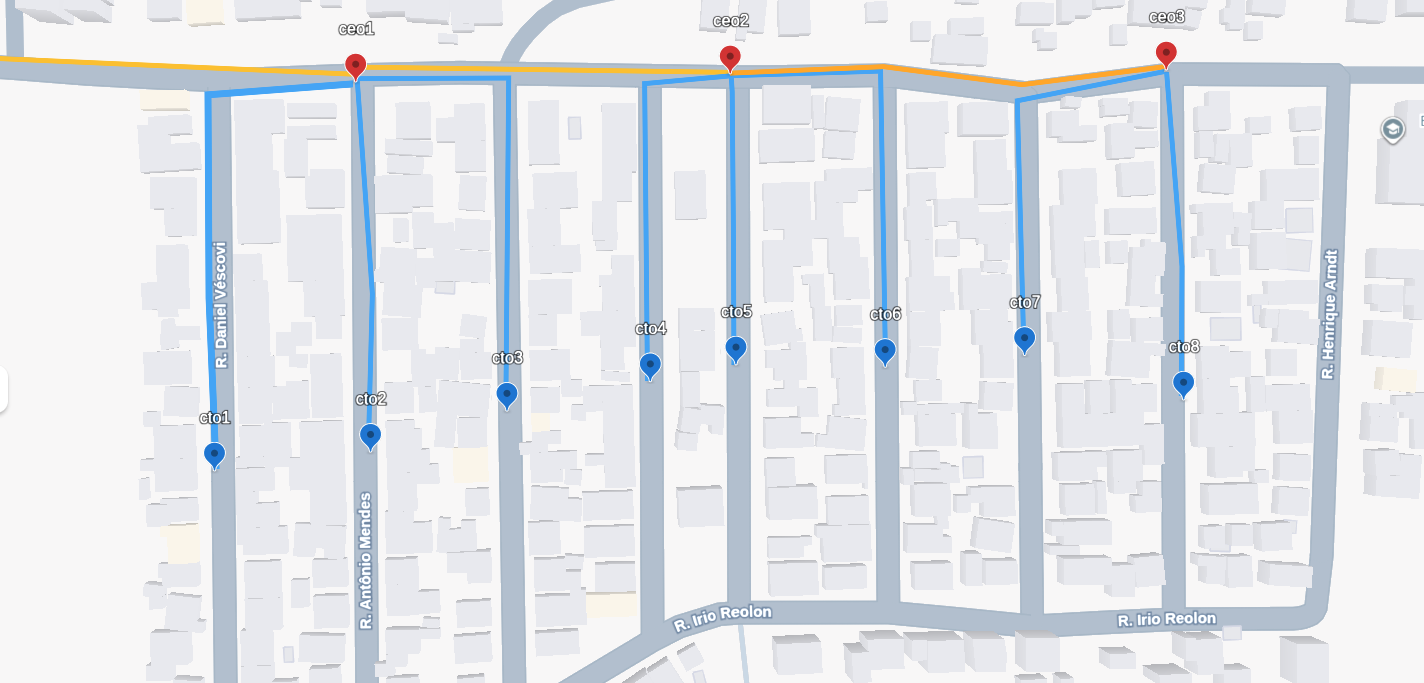
\includegraphics[width=0.9\textwidth]{images/cidade_alta_google_earth.png}
        \par\footnotesize Fonte: Elaboração própria sobre imagem do Google Earth.
    }
\end{figure}

Na abordagem tradicional via \textit{Draw.io}, a diagramação gráfica demandou 10 minutos. O cálculo manual inicial revelou forte assimetria de sinal (\glspl{onu} finais com $-16$\,dBm e iniciais com $-23$\,dBm), exigindo 45 minutos de recálculos manuais em cadeia para substituição dos \textit{splitters} desbalanceados. Para viabilizar a execução manual, desconsiderou-se a atenuação da fibra secundária e das conexões entre as caixas.

As Figuras~\ref{fig:drawio_bloco1}, \ref{fig:drawio_bloco2} e \ref{fig:drawio_bloco3} ilustram a topologia em blocos no \textit{Draw.io}.

\begin{figure}[htb]
    \caption{Bloco 1 do diagrama no \textit{Draw.io} -- OLT, CEO-1 e CTOs 1 a 3}
    \label{fig:drawio_bloco1}
    \centering
    \parbox{16cm}{
        \centering
        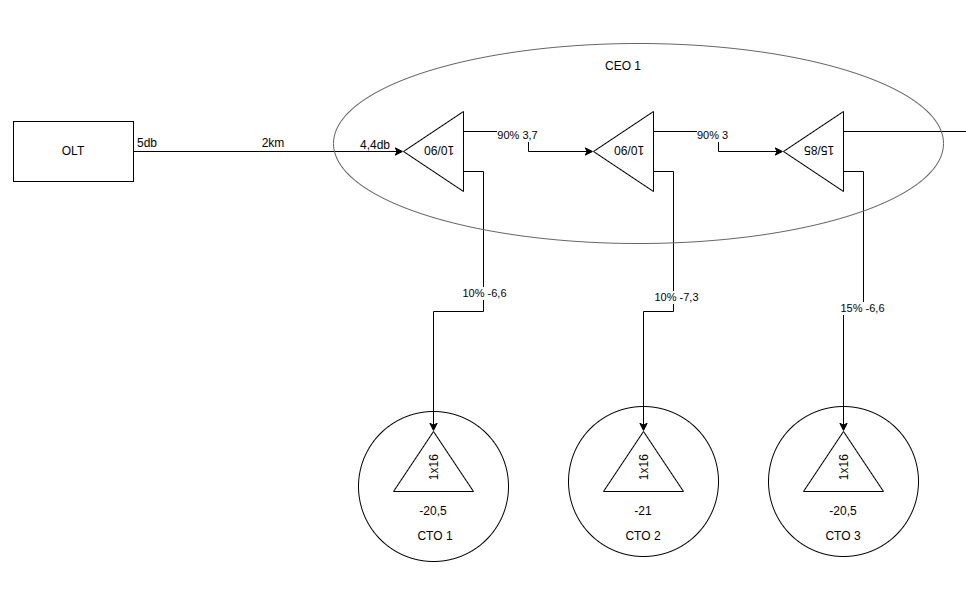
\includegraphics[width=0.9\textwidth]{images/drawio_bloco1.png}
        \par\footnotesize Fonte: Elaboração própria no Draw.io.
    }
\end{figure}

\begin{figure}[htb]
    \caption{Bloco 2 do diagrama no \textit{Draw.io} -- CEO-2 e CTOs 4 a 6}
    \label{fig:drawio_bloco2}
    \centering
    \parbox{16cm}{
        \centering
        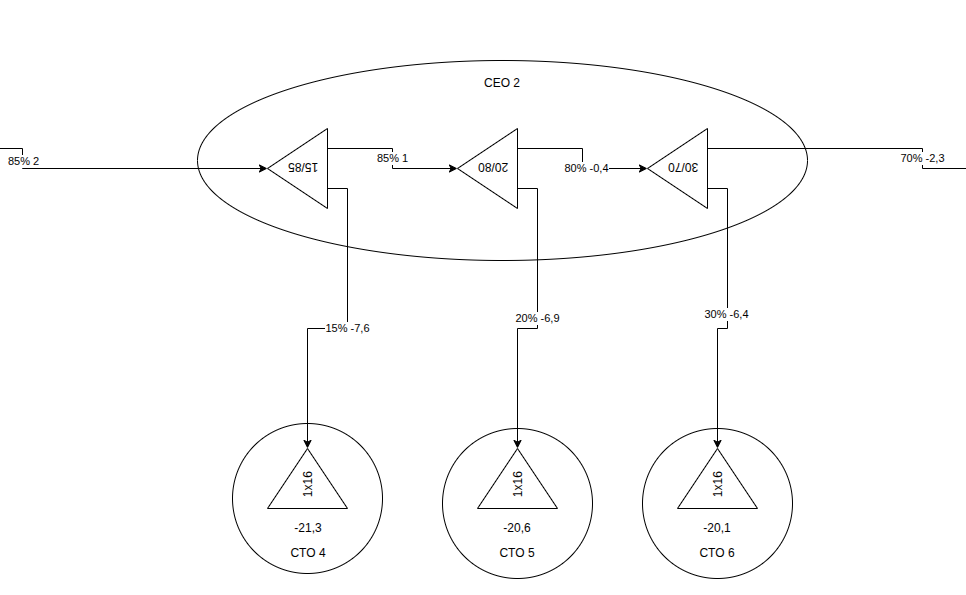
\includegraphics[width=0.9\textwidth]{images/drawio_bloco2.png}
        \par\footnotesize Fonte: Elaboração própria no Draw.io.
    }
\end{figure}

\begin{figure}[htb]
    \caption{Bloco 3 do diagrama no \textit{Draw.io} -- CEO-3 e CTOs 7 e 8}
    \label{fig:drawio_bloco3}
    \centering
    \parbox{16cm}{
        \centering
        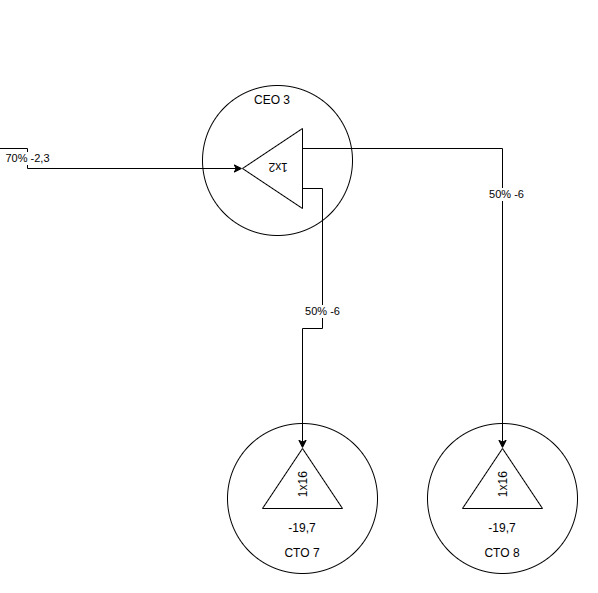
\includegraphics[width=0.9\textwidth]{images/drawio_bloco3.png}
        \par\footnotesize Fonte: Elaboração própria no Draw.io.
    }
\end{figure}

No \textit{PON Planner}, o mesmo projeto foi modelado e balanceado em apenas 10 minutos. A ferramenta computou automaticamente a atenuação real de fusões, conectores e comprimentos exatos dos cabos intermediários. As Figuras~\ref{fig:ponplanner_bloco1}, \ref{fig:ponplanner_bloco2} e \ref{fig:ponplanner_bloco3} exibem os blocos correspondentes no software.

\begin{figure}[htb]
    \caption{Bloco 1 do diagrama no \textit{PON Planner} -- OLT, CEO-1 e CTOs 1 a 3}
    \label{fig:ponplanner_bloco1}
    \centering
    \parbox{16cm}{
        \centering
        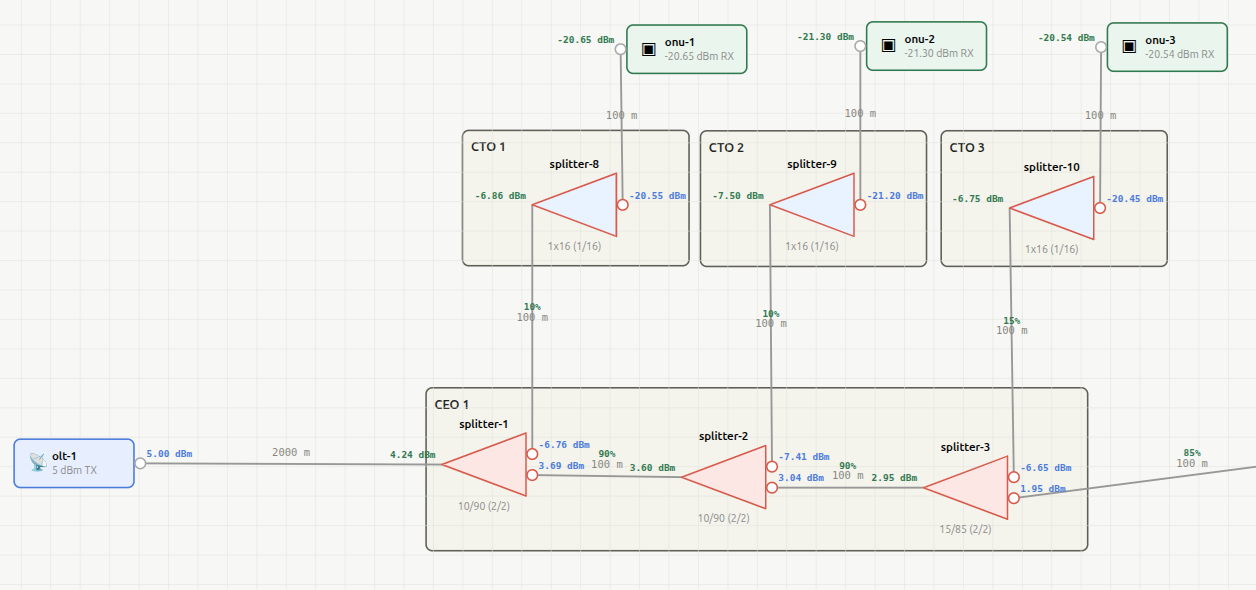
\includegraphics[width=0.9\textwidth]{images/ponplanner_bloco1.png}
        \par\footnotesize Fonte: Elaborado na aplicação PON Planner.
    }
\end{figure}

\begin{figure}[htb]
    \caption{Bloco 2 do diagrama no \textit{PON Planner} -- CEO-2 e CTOs 4 a 6}
    \label{fig:ponplanner_bloco2}
    \centering
    \parbox{16cm}{
        \centering
        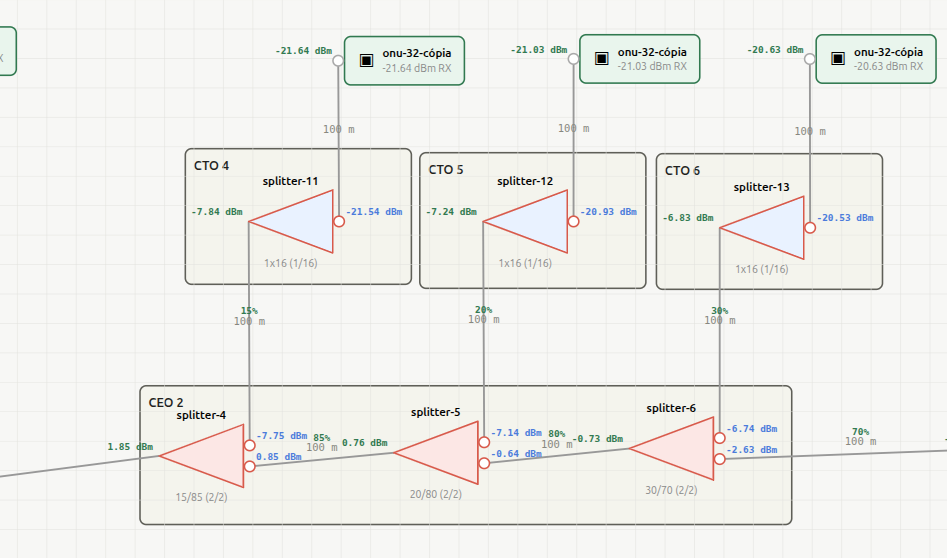
\includegraphics[width=0.9\textwidth]{images/ponplanner_bloco2.png}
        \par\footnotesize Fonte: Elaborado na aplicação PON Planner.
    }
\end{figure}

\begin{figure}[htb]
    \caption{Bloco 3 do diagrama no \textit{PON Planner} -- CEO-3 e CTOs 7 e 8}
    \label{fig:ponplanner_bloco3}
    \centering
    \parbox{16cm}{
        \centering
        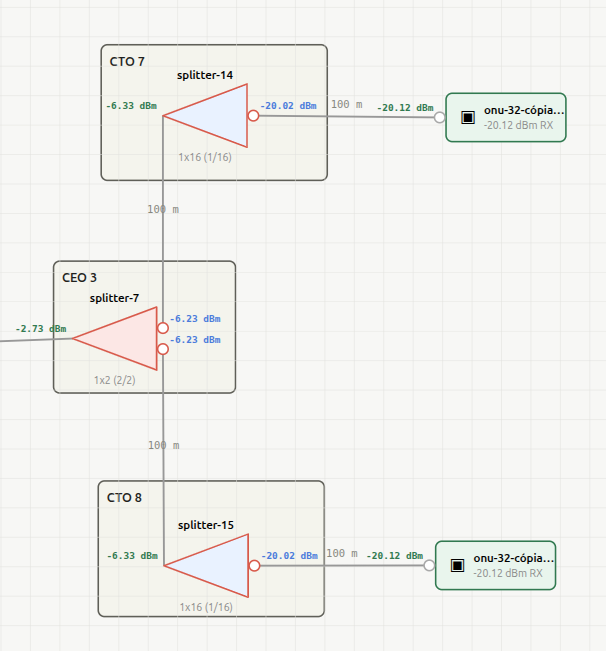
\includegraphics[width=0.9\textwidth]{images/ponplanner_bloco3.png}
        \par\footnotesize Fonte: Elaborado na aplicação PON Planner.
    }
\end{figure}

A Tabela~\ref{tab:comparativo_teste1} apresenta os dados numéricos de potência óptica recebida nas \glspl{onu} das 8 \glspl{cto}, comparando a estimativa manual simplificada com a simulação física do \textit{PON Planner}.

\begin{table}[htb]
\centering
\caption{Comparação da potência óptica recebida (dBm) por CTO no cenário de área urbana}
\label{tab:comparativo_teste1}
\small
\begin{tabular}{c c c c}
\hline
\textbf{Ponto de Atendimento} & \textbf{Cálculo Manual (dBm)} & \textbf{PON Planner (dBm)} & \textbf{Diferença (dB)} \\
\hline
CTO 1 & $-20{,}50$ & $-20{,}65$ & $+0{,}15$ \\
CTO 2 & $-21{,}00$ & $-21{,}30$ & $+0{,}30$ \\
CTO 3 & $-20{,}50$ & $-20{,}54$ & $+0{,}04$ \\
CTO 4 & $-21{,}30$ & $-21{,}64$ & $+0{,}34$ \\
CTO 5 & $-20{,}60$ & $-21{,}03$ & $+0{,}43$ \\
CTO 6 & $-20{,}10$ & $-20{,}63$ & $+0{,}53$ \\
CTO 7 & $-19{,}70$ & $-20{,}12$ & $+0{,}42$ \\
CTO 8 & $-19{,}70$ & $-20{,}12$ & $+0{,}42$ \\
\hline
\end{tabular}
\par\footnotesize Fonte: Elaborado pelo autor com base nos experimentos praticados.
\end{table}

A Tabela~\ref{tab:tempo_teste1} sintetiza o ganho de tempo obtido no Teste 1.

\begin{table}[htb]
\centering
\caption{Comparação do tempo gasto na elaboração e balanceamento do Teste 1}
\label{tab:tempo_teste1}
\begin{tabularx}{\textwidth}{X c c c}
\hline
\textbf{Etapa} & \textbf{Método Tradicional} & \textbf{PON Planner} & \textbf{Desempenho} \\
\hline
Desenho / Lançamento dos Elementos & 10 min & 7 min & Redução de 30,0\% \\
Cálculo e Balanceamento de Sinal & 45 min & 3 min & Redução de 93,3\% \\
\hline
\textbf{Tempo Total} & \textbf{55 min} & \textbf{10 min} & \textbf{Redução de 81,8\%} \\
\hline
\end{tabularx}
\par\footnotesize Fonte: Elaborado pelo autor.
\end{table}

\subsection{Teste 2 -- Estudo de Caso em Área Rural}
\label{subsec:teste2_ibirama}

O Teste 2 avaliou a aplicação em uma topologia linear de longo alcance típica de área rural, originalmente documentada em sistema de inventário georreferenciado, conforme ilustrado na Figura~\ref{fig:ibirama_geogrid}. A rede compreende 14 CTOs encadeadas ao longo de uma via principal e um cabo tronco alimentador de 9.500 metros ($\approx 9{,}5$\,km). 

Diferente do cenário urbano, a rede rural impõe um desafio de balanceamento muito mais complexo e rigoroso. Devido à grande distância percorrida pelo tronco e à distribuição espaçada das caixas, é inviável utilizar divisores balanceados simétricos em cascata sem provocar atenuação excessiva nos clientes intermediários e finais. Exige-se, portanto, a adoção de \textit{splitters} desbalanceados em cada derivação, calculando com precisão a fração de potência desviada para o atendimento local e a fração passante transmitida para o segmento seguinte.

\begin{figure}[htb]
    \caption{Mapeamento da rede óptica em área rural no sistema de inventário}
    \label{fig:ibirama_geogrid}
    \centering
    \parbox{16cm}{
        \centering
        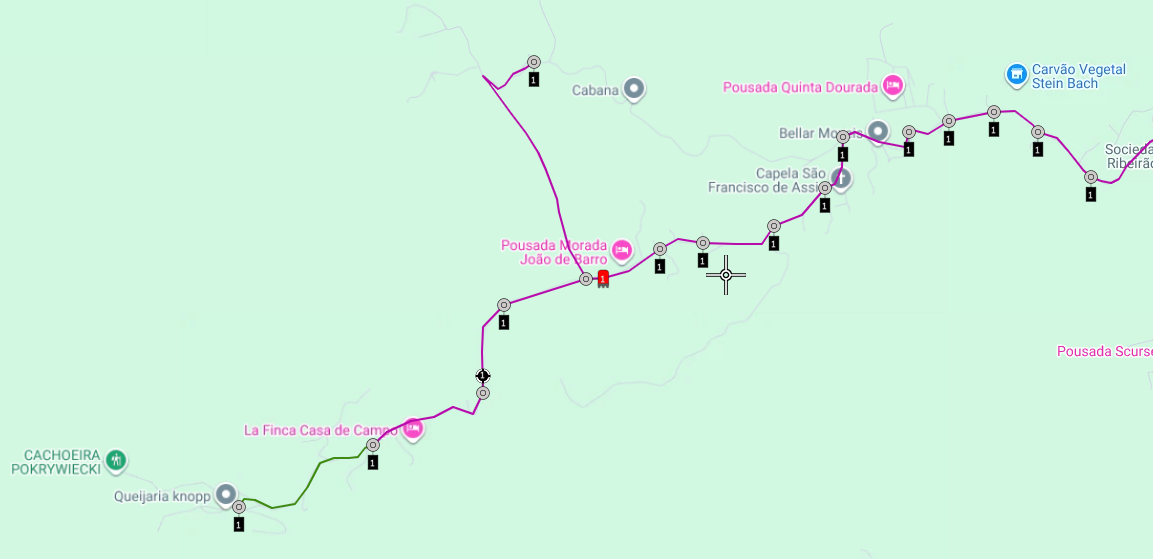
\includegraphics[width=0.9\textwidth]{images/ibirama_geogrid.png}
        \par\footnotesize Fonte: Extraído de sistema de inventário de rede óptica.
    }
\end{figure}

Na tentativa de cálculo manual desbalanceado via \textit{Draw.io} (tempo de desenho de 20 minutos), desconsideraram-se as fusões e cabos secundários. As Figuras~\ref{fig:drawio_ibirama_bloco1} e \ref{fig:drawio_ibirama_bloco2} exibem os diagramas desbalanceados no \textit{Draw.io}.

\begin{figure}[htb]
    \caption{Bloco 1 do diagrama desbalanceado no \textit{Draw.io} -- OLT, CEO e CTOs 01 a 07}
    \label{fig:drawio_ibirama_bloco1}
    \centering
    \parbox{16cm}{
        \centering
        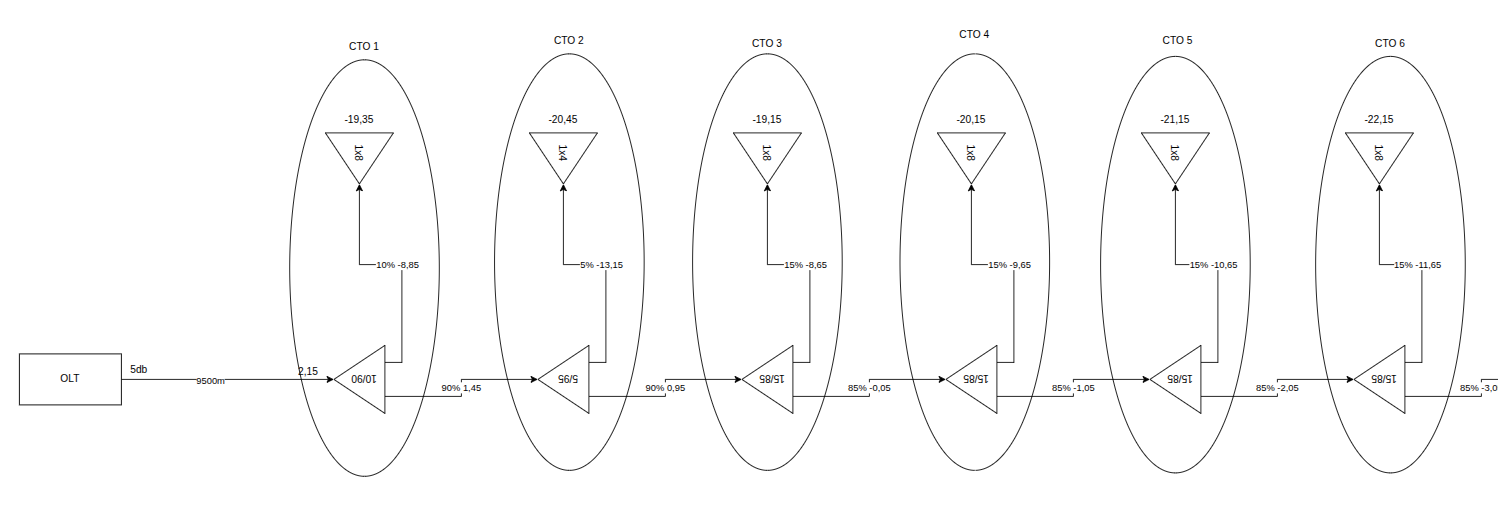
\includegraphics[width=0.9\textwidth]{images/drawio_ibirama_bloco1.png}
        \par\footnotesize Fonte: Elaborado pelo autor no Draw.io.
    }
\end{figure}

\begin{figure}[htb]
    \caption{Bloco 2 do diagrama desbalanceado no \textit{Draw.io} -- CTOs 08 a 14}
    \label{fig:drawio_ibirama_bloco2}
    \centering
    \parbox{16cm}{
        \centering
        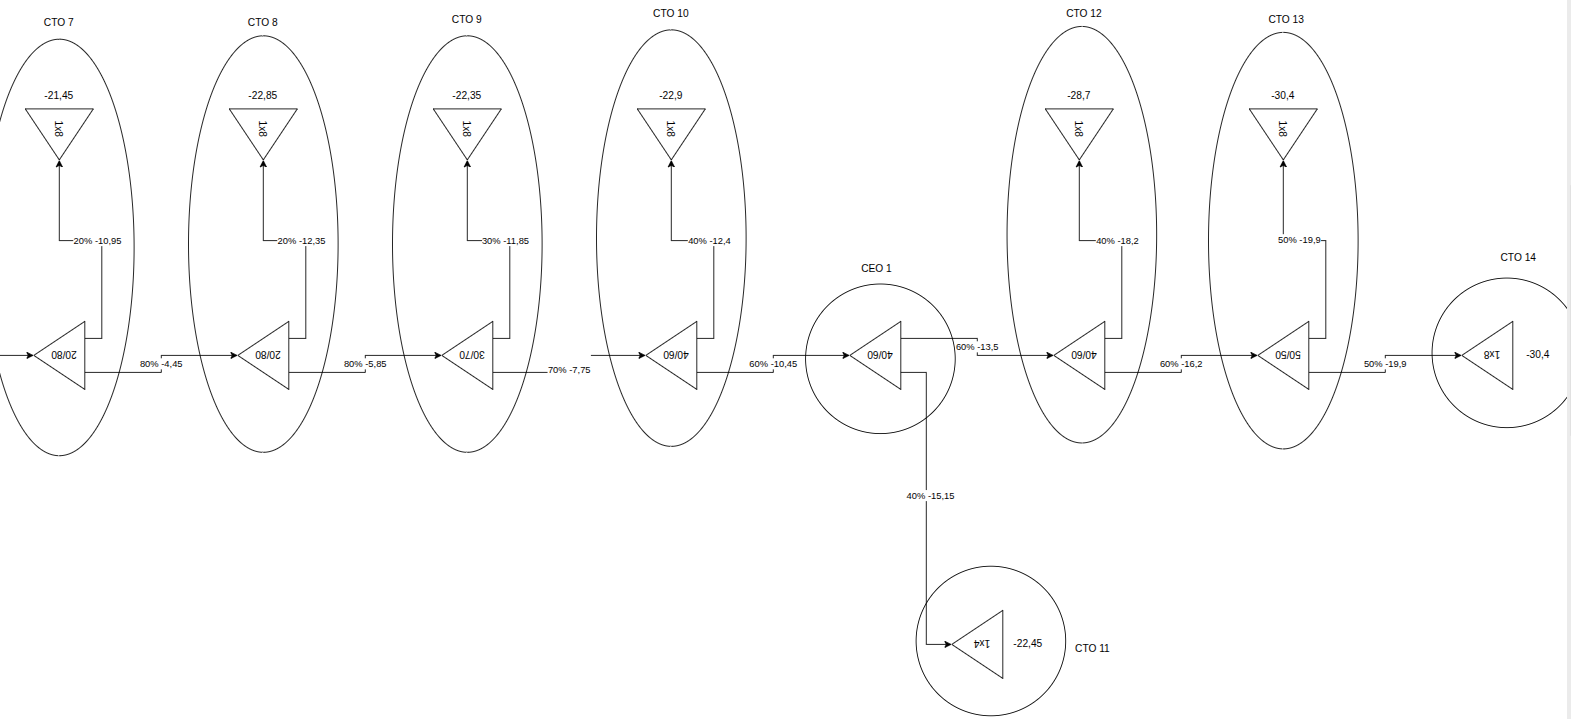
\includegraphics[width=0.9\textwidth]{images/drawio_ibirama_bloco2.png}
        \par\footnotesize Fonte: Elaborado pelo autor no Draw.io.
    }
\end{figure}

Ao simular a mesma topologia no \textit{PON Planner} (tempo de modelagem de 20 minutos), a ferramenta acusou em tempo real o colapso de sinal nos nós finais, exibindo a contagem automática dos terminais em alerta e falha. Após a identificação das falhas, executou-se o rebalanceamento no \textit{PON Planner} em apenas 5 minutos (contra estimativa superior a 90 minutos no método manual), alcançando $100\%$ das ONUs em faixa operacional verde.

As capturas do painel lateral de resumo antes e após a otimização são apresentadas lado a lado na Figura~\ref{fig:ponplanner_resumo_desbal} e na Figura~\ref{fig:ponplanner_resumo_bal}. Os diagramas completos em blocos estão disponíveis no Apêndice~\ref{apendice:diagramas_ibirama}.

\begin{figure}[htb]
    \centering
    \begin{minipage}[t]{0.45\textwidth}
        \centering
        \caption{Painel lateral na simulação desbalanceada}
        \label{fig:ponplanner_resumo_desbal}
        \vspace{0.2cm}
        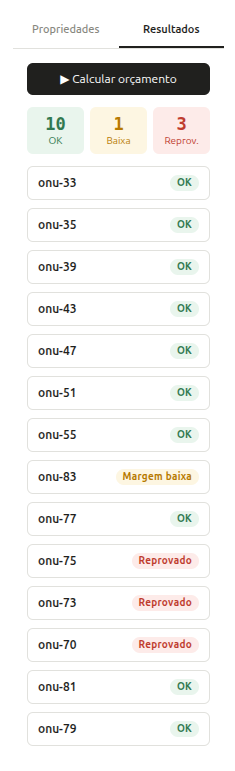
\includegraphics[width=0.55\textwidth]{images/ponplanner_resumo_desbal.png}
        \par\vspace{0.2cm}\footnotesize Fonte: Tela capturada do PON Planner.
    \end{minipage}\hfill
    \begin{minipage}[t]{0.45\textwidth}
        \centering
        \caption{Painel lateral após a otimização balanceada}
        \label{fig:ponplanner_resumo_bal}
        \vspace{0.2cm}
        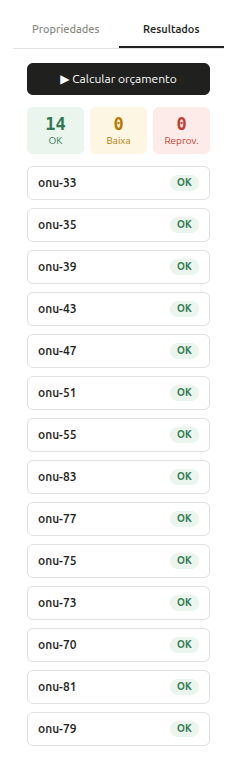
\includegraphics[width=0.55\textwidth]{images/ponplanner_resumo_bal.png}
        \par\vspace{0.2cm}\footnotesize Fonte: Tela capturada do PON Planner.
    \end{minipage}
\end{figure}

A Tabela~\ref{tab:comparativo_teste2} consolida os dados numéricos coletados nas 14 \glspl{cto} nos três cenários: estimativa manual desbalanceada, cálculo físico real desbalanceado no \textit{PON Planner} e solução final balanceada no software.

\begin{table}[htb]
\centering
\caption{Potência óptica (dBm) por CTO no cenário de área rural}
\label{tab:comparativo_teste2}
\small
\begin{tabularx}{\textwidth}{c *{3}{>{\centering\arraybackslash}X} c}
\hline
\textbf{CTO} & \textbf{Manual Desbal. (dBm)} & \textbf{PON Planner Desbal. (dBm)} & \textbf{PON Planner Bal. (dBm)} & \textbf{Status Final} \\
\hline
CTO 01 & $-19{,}35$ & $-20{,}70$ & $-23{,}68$ & OK \\
CTO 02 & $-20{,}45$ & $-21{,}02$ & $-20{,}83$ & OK \\
CTO 03 & $-19{,}15$ & $-19{,}77$ & $-20{,}98$ & OK \\
CTO 04 & $-20{,}15$ & $-20{,}87$ & $-21{,}63$ & OK \\
CTO 05 & $-21{,}15$ & $-21{,}96$ & $-22{,}27$ & OK \\
CTO 06 & $-22{,}15$ & $-23{,}06$ & $-22{,}92$ & OK \\
CTO 07 & $-21{,}45$ & $-22{,}45$ & $-23{,}57$ & OK \\
CTO 08 & $-22{,}85$ & $-23{,}95$ & $-22{,}81$ & OK \\
CTO 09 & $-22{,}35$ & $-23{,}55$ & $-23{,}91$ & OK \\
CTO 10 & $-22{,}90$ & $-24{,}24$ & $-23{,}30$ & OK \\
CTO 11 & $-22{,}45$ & $-23{,}73$ & $-23{,}20$ & OK \\
CTO 12 & $\mathbf{-28{,}70}$ \textbf{(Alerta)} & $\mathbf{-29{,}83}$ \textbf{(Falha)} & $-23{,}99$ & OK \\
CTO 13 & $\mathbf{-30{,}40}$ \textbf{(Falha)} & $\mathbf{-31{,}43}$ \textbf{(Falha)} & $-23{,}48$ & OK \\
CTO 14 & $\mathbf{-30{,}40}$ \textbf{(Falha)} & $\mathbf{-31{,}43}$ \textbf{(Falha)} & $-23{,}48$ & OK \\
\hline
\end{tabularx}
\par\footnotesize Fonte: Elaborado pelo autor com base nos dados experimentais.
\end{table}

A Tabela~\ref{tab:tempo_teste2} sintetiza a comparação de tempo no Teste 2.

\begin{table}[htb]
\centering
\caption{Comparação do tempo de execução no Teste 2 (Rede Rural de 14 CTOs)}
\label{tab:tempo_teste2}
\begin{tabularx}{\textwidth}{X c c c}
\hline
\textbf{Etapa} & \textbf{Método Tradicional} & \textbf{PON Planner} & \textbf{Desempenho} \\
\hline
Modelagem / Lançamento Gráfico & 20 min & 20 min & Equivalente \\
Cálculo e Rebalanceamento de Sinal & $> 90$ min & 5 min & \textbf{Redução $> 94,4\%$} \\
\hline
\textbf{Tempo Total de Projeto} & \textbf{$> 110$ min} & \textbf{25 min} & \textbf{Redução de $\approx 77,2\%$} \\
\hline
\end{tabularx}
\par\footnotesize Fonte: Elaborado pelo autor.
\end{table}

\section{Análise e Discussão}
\label{sec:analise_discussao}

A interpretação conjunta dos dados coletados nos estudos de caso permite discutir a fidelidade física da modelagem, o ganho real de produtividade, o alinhamento com a literatura e as limitações do protótipo.

\subsection{Interpretação dos Achados e Fidelidade Física do Cálculo}

A análise da Tabela~\ref{tab:comparativo_teste2} evidencia o risco associado a simplificações manuais de cálculo. Na \gls{cto}~01 do Teste 2, enquanto o método manual estimou $-19{,}35$\,dBm, o \textit{PON Planner} apurou $-20{,}70$\,dBm (diferença de $1{,}35$\,dB). Na \gls{cto}~12, a estimativa manual de $-28{,}70$\,dBm sugeria um nó em faixa de alerta de sensibilidade, porém a contabilização das fusões e atenuação dos conectores efetuada pelo \textit{software} revelou que o sinal real era de $-29{,}83$\,dBm (\textit{status} de Falha).

Essa divergência demonstra que abordagens manuais simplificadas podem induzir o projetista a aprovar projetos que apresentariam instabilidade ou inoperância na implantação física. O \textit{PON Planner} elimina esse viés ao computar todas as perdas distribuídas e concentradas sem impor carga de trabalho matemática ao usuário.

Além da precisão, o ganho de produtividade foi expressivo. A redução do tempo total de projeto em $81{,}8\%$ no Teste 1 e $77{,}2\%$ no Teste 2 decorre da eliminação do recálculo manual em cadeia. A reatividade do motor em Python (respostas em $<15$\,ms) transformou a busca pela combinação ideal de \textit{splitters} desbalanceados em um processo exploratório visual de poucos minutos.

\subsection{Comparação com Trabalhos Relacionados}

Os resultados obtidos reforçam o posicionamento da solução frente aos correlatos analisados no Capítulo 3:

\begin{itemize}
    \item \textbf{Em relação a \textit{softwares} de inventário \gls{gis} (GeoGrid Maps, OZmap, FTTH Planner):} Enquanto essas ferramentas privilegiam a representação cartográfica e a documentação cadastral dos ativos implantados \cite{geogridmaps2026,ozmap2026,ftthplanner2026}, o \textit{PON Planner} atua na fase de concepção técnica e planejamento lógico, integrando o cálculo dinâmico de atenuação ao desenho da topologia.
    \item \textbf{Em relação a estudos de visualização web (\citeonline{fatahillah2025visnetwork_ftth}):} Enquanto propostas acadêmicas anteriores focavam na renderização visual de grafos sem acoplamento a motores matemáticos do domínio, o \textit{PON Planner} integra a biblioteca D3.js a um motor de cálculo óptico em tempo real.
\end{itemize}

\subsection{Limitações da Solução}

Apesar dos resultados positivos, identificaram-se limitações técnicas no protótipo desenvolvido:
\begin{enumerate}
    \item \textbf{Cálculo Unidirecional (\textit{Downstream}):} O motor de cálculo processa a atenuação óptica exclusivamente no sentido \textit{downstream} (\gls{olt} $\rightarrow$ \gls{onu}). Embora o canal de descida concentre as maiores taxas de divisão em \textit{splitters}, o dimensionamento completo exige avaliar também o orçamento do canal de \textit{upstream} (1310\,nm).
    \item \textbf{Ausência de Camada \gls{gis} Integrada:} O sistema opera focado na topologia lógica ponto-multiponto. A determinação dos comprimentos físicos dos cabos exige o uso de ferramentas de apoio externo (como \textit{Google Earth} ou \textit{GeoGrid Maps}) para posterior inserção na propriedade dos enlaces.
    \item \textbf{Persistência Local e Monousuário:} O armazenamento dos projetos em arquivos \gls{json} no sistema de arquivos local atende a cenários individuais, mas não suporta edição colaborativa simultânea ou controle de concorrência.
\end{enumerate}

\section{Validação dos Objetivos}
\label{sec:validacao_objetivos}

Para assegurar o rigor metodológico da pesquisa, esta seção verifica o cumprimento sistemático dos objetivos propostos na Introdução.

\subsection{Cumprimento dos Objetivos Específicos}

A Tabela~\ref{tab:validacao_objetivos_especificos} estabelece a correspondência direta entre cada objetivo específico definido no Capítulo 1 e as evidências de implementação e resultados obtidos no trabalho.

\begin{table}[htb]
\centering
\caption{Quadro de verificação do cumprimento dos Objetivos Específicos}
\label{tab:validacao_objetivos_especificos}
\small
\begin{tabularx}{\textwidth}{|p{3.2cm}|p{4.6cm}|X|c|}
\hline
\textbf{Objetivo Específico} & \textbf{Funcionalidade / Artefato} & \textbf{Evidência nos Resultados} & \textbf{Status} \\
\hline
1. Modelagem visual de topologias \gls{pon} com inserção e edição de nós e enlaces. & Interface web \textit{SPA} com biblioteca D3.js e manipuladores de \textit{drag-and-drop}. & Demonstração prática nos Testes 1 e 2 (Figuras~\ref{fig:ponplanner_bloco1} a \ref{fig:ponplanner_bloco3}). & \textbf{Alcançado} \\
\hline
2. Cálculo automático do orçamento óptico considerando perdas de fibra, conectores, fusões e \textit{splitters}. & Motor de cálculo em Python (\texttt{calculo\_optico.py}) baseado em travessia \gls{dfs}. & Tabelas~\ref{tab:comparativo_teste1} e \ref{tab:comparativo_teste2} com precisão física detalhada. & \textbf{Alcançado} \\
\hline
3. Apresentação de indicadores de potência, margem e \textit{status} dos enlaces. & Código de cores nos nós (verde/amarelo/vermelho) e painel lateral de resumo. & Figuras~\ref{fig:ponplanner_resumo_desbal} e \ref{fig:ponplanner_resumo_bal} no Teste 2 (RF5). & \textbf{Alcançado} \\
\hline
4. Persistência, recuperação e troca de projetos em formato \gls{json}. & Esquema Pydantic (\texttt{network.py}) e serviço \texttt{ProjetoService}. & Estrutura JSON validada na Seção~\ref{sec:modelagem_dados} e arquivos em \texttt{data/projects}. & \textbf{Alcançado} \\
\hline
\end{tabularx}
\par\footnotesize Fonte: Elaborado pelo autor.
\end{table}

\subsection{Análise do Cumprimento do Objetivo Geral}

O \textbf{Objetivo Geral} deste trabalho consistia em \textit{``desenvolver uma aplicação web interativa que integre a modelagem visual da topologia de redes ópticas \gls{pon} ao cálculo automático do orçamento óptico, fornecendo uma solução que auxilie o planejamento, a análise e a validação técnica de projetos de redes \gls{ftth}''}.

Conforme demonstrado ao longo do desenvolvimento (Capítulo 5) e validado nos estudos de caso (Capítulo 6), a solução \textit{PON Planner} integrou com sucesso a modelagem gráfica de grafos ao cálculo dinâmico de perdas em tempo real. A ferramenta comprovou sua capacidade de elevar a precisão física do planejamento, eliminar falhas de diagnóstico causadas por simplificações manuais e reduzir o tempo total de elaboração e balanceamento de projetos \gls{gpon} em mais de $77\%$. Desse modo, conclui-se que o Objetivo Geral foi \textbf{plenamente alcançado}.